% metodologia
\chapter{Metodologia}
\thispagestyle{fancy}

A elaboração do presente trabalho se deu em 3 etapas distintas:

\begin{enumerate}
	\item Estudo de viabilidade do \emph{Website Parse Template} (WPT) como \emph{Domain Specific Language} (DSL) para \emph{web scrapers}, assim como busca de melhores alternativas.
	\item Estudo do funcionamento e arquitetura do framework Scrapy.
	\item Implementação de uma ferramenta e seus respectivos testes automatizados para compilação do WPT em um \emph{spider} do Scrapy.
\end{enumerate}

A seguir, é mostrada uma descrição mais detalhada de cada etapa de produção deste trabalho.

\section{Estudo de viabilidade do WPT e outras alternativas}

Uma preocupação constante no desenvolvimento do presente trabalho foi a procura por adoção de padrões abertos que sejam amplamente utilizados.

Além do Website Parse Template, outras duas alternativas foram pesquisadas: o Protocol Buffer \cite{protobuf} e o JSON \cite{JSON}. Ambas foram descartadas pelos motivos citados anteriormente ao passo que o WPT se encaixou bem na lista de requisitos.

\section{Estudo do Scrapy}

Uma das grandes vantagens percebidas do framework Scrapy é a sua abundante documentação, seja a oficial em documentos HTML ou a documentação disponível dentro do próprio código fonte do mesmo.

Os principais itens estudados foram a geração de código, comandos disponíveis na linha de comando, testes unitários automatizados e estratégias de desenvolvimento.

O Scrapy possui uma coleção de testes automatizados, que permitem um melhor entendimento do framewok ao observar o que e como os componentes do mesmo estão sendo testados. Além disso, os testes disponíveis fornecem um esquema pré-definido de como os testes para novas funcionalidades deverão ser feitos. Os testes desta ferramenta se encontram no pacote \texttt{scrapy.tests.test\_commands}, ao passo que sua implementação se encontra em \\
 \texttt{scrapy.commands.importwpt}.

\section{Desenvolvimento da ferramenta}

O Scrapy possui um utilitário de linha de comando que permite a criação de novos projetos de \emph{web scrapers}, assim como sua execução, manutenção e observação de funcionamento do projeto. O exemplo mostrado na Listagem \ref{scrapy_saida_comando_scrapy} ilustra a saída da execução do comando "scrapy":

\lstset{basicstyle=\scriptsize,
caption={Saída da execução do comando ''scrapy''},
captionpos=b
}
\begin{lstlisting}[label=scrapy_saida_comando_scrapy]
Scrapy 0.11 - no active project

Usage:
  scrapy <command> [options] [args]

Available commands:
  fetch         Fetch a URL using the Scrapy downloader
  runspider     Run a self-contained spider (without creating a project)
  settings      Get settings values
  shell         Interactive scraping console
  startproject  Create new project
  version       Print Scrapy version
  view          Open URL in browser, as seen by Scrapy

Use "scrapy <command> -h" to see more info about a command
\end{lstlisting}

A ferramenta desenvolvida neste trabalho foi incluída no comando apresentado anteriormente e pode ser observado quando o Scrapy detecta que está dentro de uma pasta de projeto como demonstrado na Listagem \ref{scrapy_comando_pasta_projeto}.

\pagebreak
\lstset{basicstyle=\scriptsize,
caption={Saída da execução do comando ''scrapy'' dentro da pasta de um projeto},
captionpos=b
}
\begin{lstlisting}[label=scrapy_comando_pasta_projeto]
Scrapy 0.11 - project: scrapytest

Usage:
  scrapy <command> [options] [args]

Available commands:
  crawl         Start crawling from a spider or URL
  deploy        Deploy project in Scrapyd server
  fetch         Fetch a URL using the Scrapy downloader
  genspider     Generate new spider using pre-defined templates
  importwpt     Create a spider based on a Website Parse Template (WPT) file
  list          List available spiders
  parse         Parse URL (using its spider) and print the results
  queue         Control execution queue
  runserver     Start Scrapy in server mode
  runspider     Run a self-contained spider (without creating a project)
  settings      Get settings values
  shell         Interactive scraping console
  startproject  Create new project
  version       Print Scrapy version
  view          Open URL in browser, as seen by Scrapy

Use "scrapy <command> -h" to see more info about a command

\end{lstlisting}

O comando \texttt{importwpt} cd lê um arquivo XML utilizando o formato WPT e cria um \emph{spider} do scrapy a partir dele. Após isso, a execução do comando \texttt{scrapy crawl nome\_do\_spider\_gerado} irá executar o processo de extração de informações conforme descrito no XML que foi importado.

Dentre todos os elementos e seus atributos que a especificação do WPT apresenta, não há nenhum que diz sobre o tratamento e armazenamento dos dados obtidos. Por este motivo, somente a especificação do WPT é insuficiente para construir um sistema de recuperação de informações completo. Por exemplo, o atributo não-oficial \texttt{name} dentro da tag \texttt{<ow:block>} é necessário para nomeação de objetos dentro do \emph{spider}, como demonstrado na listagem \ref{scrapy_conteudo_arquivo_entrada}.

\lstset{language=XML,
basicstyle=\scriptsize,
caption={Conteúdo do arquivo de entrada para o comando \texttt{scrapy importwpt}},
captionpos=b
}
\begin{lstlisting}[label=scrapy_conteudo_arquivo_entrada]
  <ow:wpt xmlns:ow="http://www.omfica.org/schemas/ow/0.9"
            ow:host="http://example.com">
  <ow:template ow:name="Template Example" ow:url="http://www.example.com/index.php">
      <ow:block ow:tagid="ex1" name="ex1"></ow:block>
  </ow:template> 
  </ow:wpt>
\end{lstlisting}

Como o principal objetivo deste trabalho é facilitar a criação e manutenção de sistemas de recuperação de informação, não é desejável ter nomes de variáveis geradas aleatoriamente no processo de conversão do WPT para o spider do Scrapy. Observa-se, então, o uso do conteúdo do atributo \texttt{name} no código gerado, como mostrado na listagem \ref{scrapy_spider_gerado}.

\lstset{language=Python,
basicstyle=\scriptsize,
caption={\emph{Spider} gerado a partir do arquivo de entrada apresentado na listagem 5.3},
captionpos=b
}
\begin{lstlisting}[label=scrapy_spider_gerado]
from scrapy.item import Item, Field

class TemplateExampleItem1(Item):
    ex1 = Field()

from scrapy.spider import BaseSpider
from scrapy.contrib.loader import XPathItemLoader

class TemplateExample(BaseSpider):
    name = 'example.com'
    allowed_domains = ['example.com']
    start_urls = [
        'http://www.example.com/index.php',
    ]

    def parse(self, response):
        l = XPathItemLoader(item = TemplateExampleItem1(),response=response)
        l.add_xpath('bubble','id("ex1")/text()') 
        i = l.load_item()
        yield i

\end{lstlisting}


Como este trabalho ainda está em andamento, algumas funcionalidades, tais como exportação dos dados obtidos, não estão presentes. Por ser um projeto de código aberto, há a possibilidade desta ferramenta ser desenvolvido por outras pessoas e mais funcionalidades serem adicionadas com o passar do tempo.

No entanto, no que tange á criação de \emph{spiders}, o projeto funciona conforme as especificações do WPT (disponíveis em \cite{wpt}). Como estas especificações ainda estão em desenvolvimento, é possível que em um futuro próximo seja necessária a manutenção do projeto a fim de ser compatível com a última versão do WPT.

\subsection{Versionamento do código}

Todo o código da ferramenta foi versionado utilizando o Git. O uso do Git, juntamente com a hospedagem provida pelo Github, facilita a organização, colaboração e diminui os riscos de perda total ou parcial do trabalho diante de várias interpéries externas, como furto ou inutilização de equipamentos, acidentes e erros humanos.

O utilitário \texttt{gitk} permite uma melhor visualização do trabalho feito, assim como o acompanhamento das mudanças ao longo do tempo, como mostrado na Figura \ref{gitk}:

\begin{figure} [ht]
	\begin{center}
		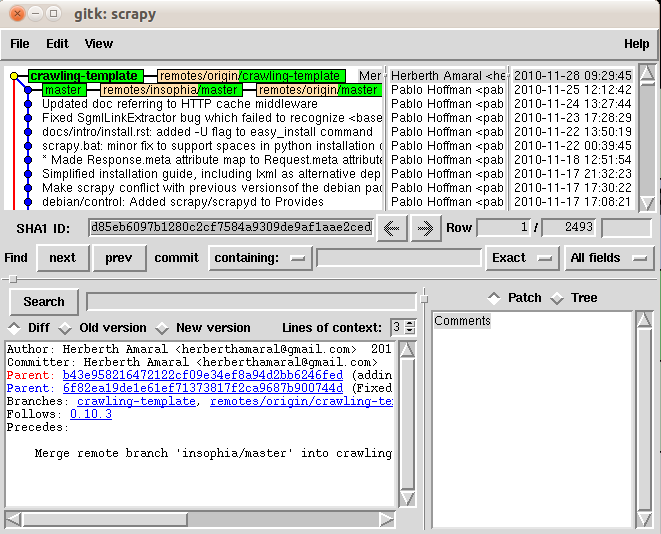
\includegraphics[scale=0.5]{gitk.png}
	\end{center}
	\caption{Visualização dos detalhes do repositório de código da ferramenta desenvolvida com o utilitário Gitk}
	\label{gitk}
\end{figure}

\pagebreak
Este trabalho também pôde ser acompanhado por outras pessoas que não fazem parte dele diretamente através do Github. No Github, ferramentas como o \emph{Graph Viewer} permite uma visualição do trabalho desenvolvido, como mostrado na Figura \ref{github}:

\begin{figure} [ht]
	\begin{center}
		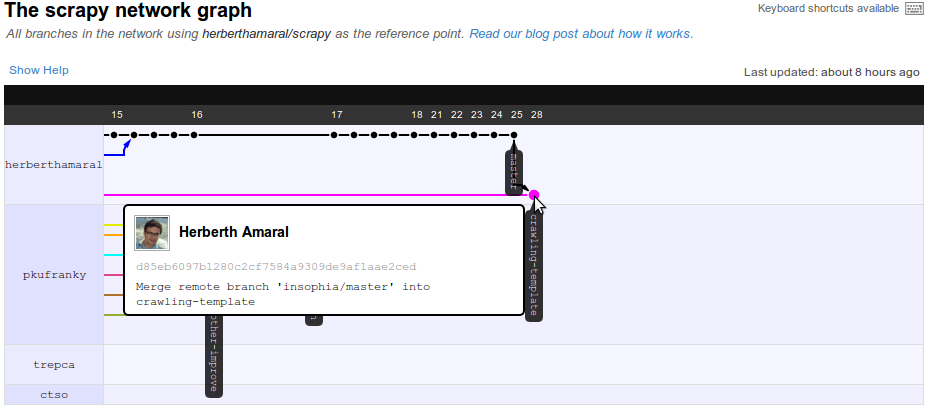
\includegraphics[scale=0.5]{github.png}	
	\end{center}
	\caption{Visualização online dos detalhes do repositório de código da ferramenta desenvolvida no Github}
	\label{github}
\end{figure}

